\chapter{Implementación}\label{cap:implementacion}

En este apartado se describirá la solución final implementada, detallando tanto el pipeline de procesamiento de imágenes, como la interfaz gráfica desarrollada junto con una breve guía de uso. Para ello, se dividirá el capítulo en dos secciones: una dedicada al backend y otra al frontend.

\section{Backend}

El backend de la aplicación se encarga de procesar las imágenes de alta velocidad obtenidas durante los experimentos con nebulizadores Flow Blurring. Para ello, se ha desarrollado un pipeline de procesamiento que incluye varias etapas, como la preprocesamiento de las imágenes, la segmentación de las gotas y la extracción de características relevantes para el análisis.

Cabe destacar que la mayor parte del esfuerzo de implementación se ha centrado en el desarrollo de este pipeline de procesamiento, ya que es la parte más crítica y compleja de la aplicación. Se han utilizado diversas técnicas de procesamiento de imágenes, como filtros de suavizado, umbralización adaptativa y algoritmos de detección de bordes, para lograr una segmentación precisa de las gotas.

\subsection{Arquitectura del Analizador}

El procesamiento de imágenes se ha implementado en una clase llamada \texttt{DropletAnalyzer}, que se encarga de recibir un vídeo de alta velocidad, procesar cada uno de sus frames y extraer las características relevantes de las gotas presentes en cada frame. El resultado final se almacena en un formato estructurado que puede ser utilizado para análisis posteriores.

Dicha clase se ha diseñado de forma modular, permitiendo la fácil incorporación de nuevas técnicas de procesamiento o la modificación de las existentes sin afectar al resto del pipeline. Esto dota a la aplicación de una gran flexibilidad, permitiendo seleccionar diferentes técnicas de preprocesamiento o segmentación según las características específicas de los vídeos a analizar. Es decir, podríamos definir el pipeline como una cadena de bloques que reciben un frame, ejecutan una acción sobre él y lo pasan al siguiente bloque, de forma que cada bloque es independiente del resto y se pueden modificar o sustituir sin afectar a los demás. La figura \ref{fig:diagramaPipeline} muestra un diagrama de alto nivel donde se pueden diferenciar las distintas etapas (los bloques) por las que pasa cada frame del vídeo hasta obtener el resultado final.

\begin{figure}[ht] 
    \centering
    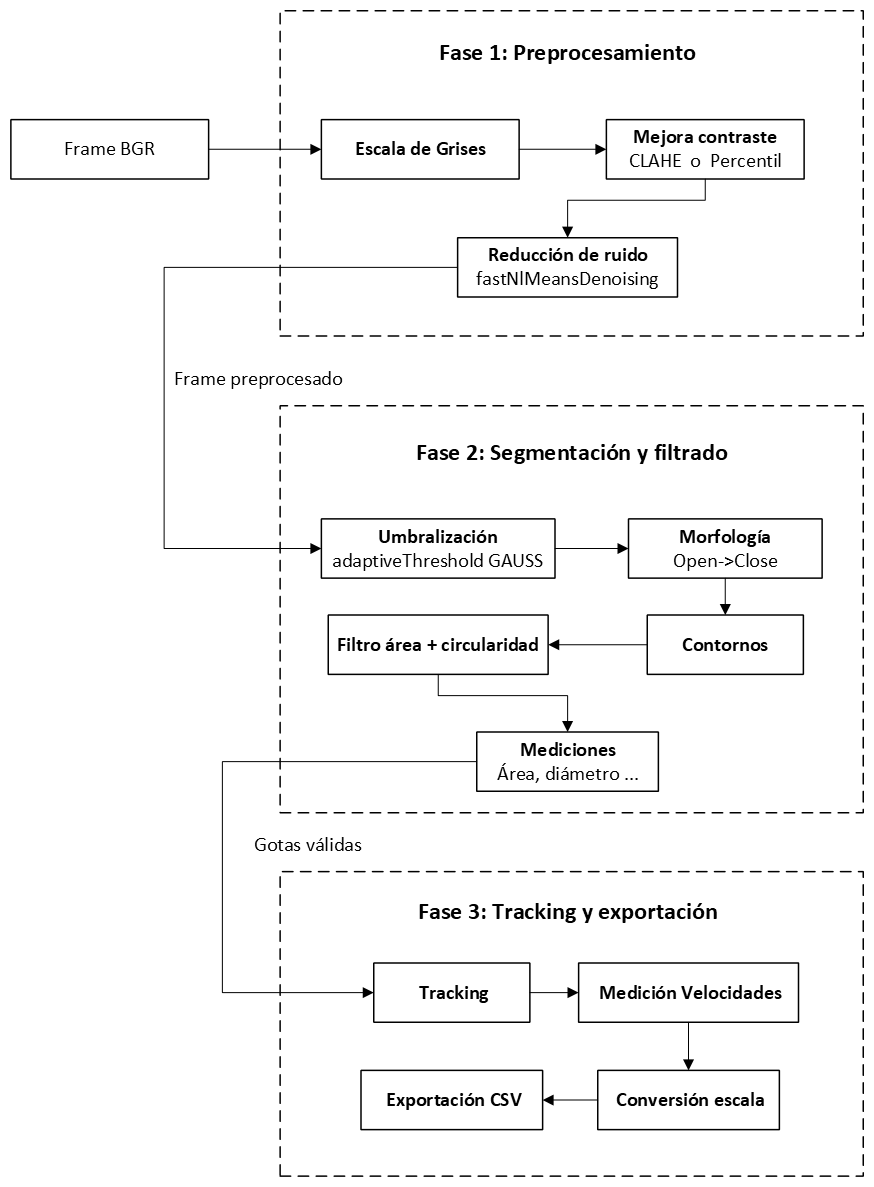
\includegraphics[width=1\textwidth]{figures/Diagrama1.png}
    \caption{Diagrama del pipeline de procesamiento.}
    \label{fig:diagramaPipeline}
\end{figure}

\FloatBarrier

También se han tenido que definir tres tipos de datos (diccionarios) para poder almacenar los parámetros que el usuario puede configurar en la interfaz gráfica, los resultados del procesamiento de cada frame y los resultados finales, una vez terminado el tracking. En la figura \ref{fig:diagramaClaseAn} se muestra un diagrama de la clase \texttt{DropletAnalyzer}, donde se pueden observar los atributos que almacenan estos datos, así como los métodos principales que se encargan de ejecutar cada una de las etapas del pipeline de procesamiento.

\subsection{Preprocesamiento}

El preprocesamiento de los frames del vídeo es la primera etapa del pipeline implementado. En esta etapa se aplican diversas técnicas para mejorar la calidad del contraste y la reducción de ruido en las imágenes, facilitando así la posterior segmentación de las gotas.

Como se pude apreciar en el diagrama de la figura \ref{fig:diagramaPipeline}, el preprocesamiento se compone de tres etapas principales: la conversión a escala de grises, la mejora del contraste y la reducción de ruido. Veamos cada uno de estos bloques con más detalle.

\subsubsection{Conversión a escala de grises}

Como vimos en la sección \ref{sec:intropi}, las imágenes pueden estar compuestas por múltiples canales de color, en nuestro caso, los vídeos de alta velocidad están en formato RGB, aunque el vídeo se vea en blanco y negro. Al pasar de los tres canales RGB de los frames originales a un canal de escala de grises, se simplifica el procesamiento y se reduce la cantidad de información a manejar. Además los algoritmos de detección de bordes usados pasan internamente las imágenes a escala de grises, por lo que no estamos perdiendo ninguna información.

Para realizar esta transformación se usa la función \texttt{cv2.cvtColor} de OpenCV. En las siguientes figuras se muestra el antes y después de la conversión, aunque a simple vista  es difícil apreciar la diferencia.

\begin{figure}[ht]
    \centering
    \begin{subfigure}[t]{0.35\textwidth}
        \centering
        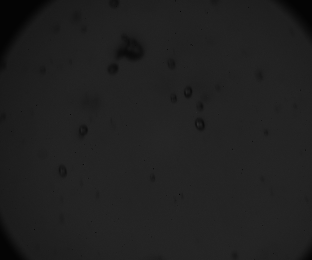
\includegraphics[width=\textwidth]{figures/frameoriginal.png}
        \caption{Original}  
        \label{subfig:original}
    \end{subfigure}
    \hfill
    \begin{subfigure}[t]{0.35\textwidth}
        \centering
        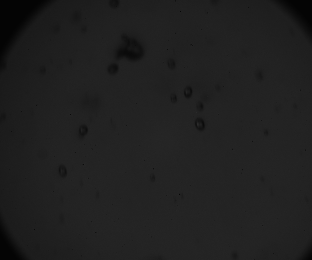
\includegraphics[width=\textwidth]{figures/escaladegrises.png}
        \caption{Gray}  
        \label{subfig:gris}
    \end{subfigure}
    
    \caption{Conversión a escala de grises.}
    \label{fig:preproc-gris}
\end{figure}
\FloatBarrier
\begin{figure}[ht] 
    \centering
    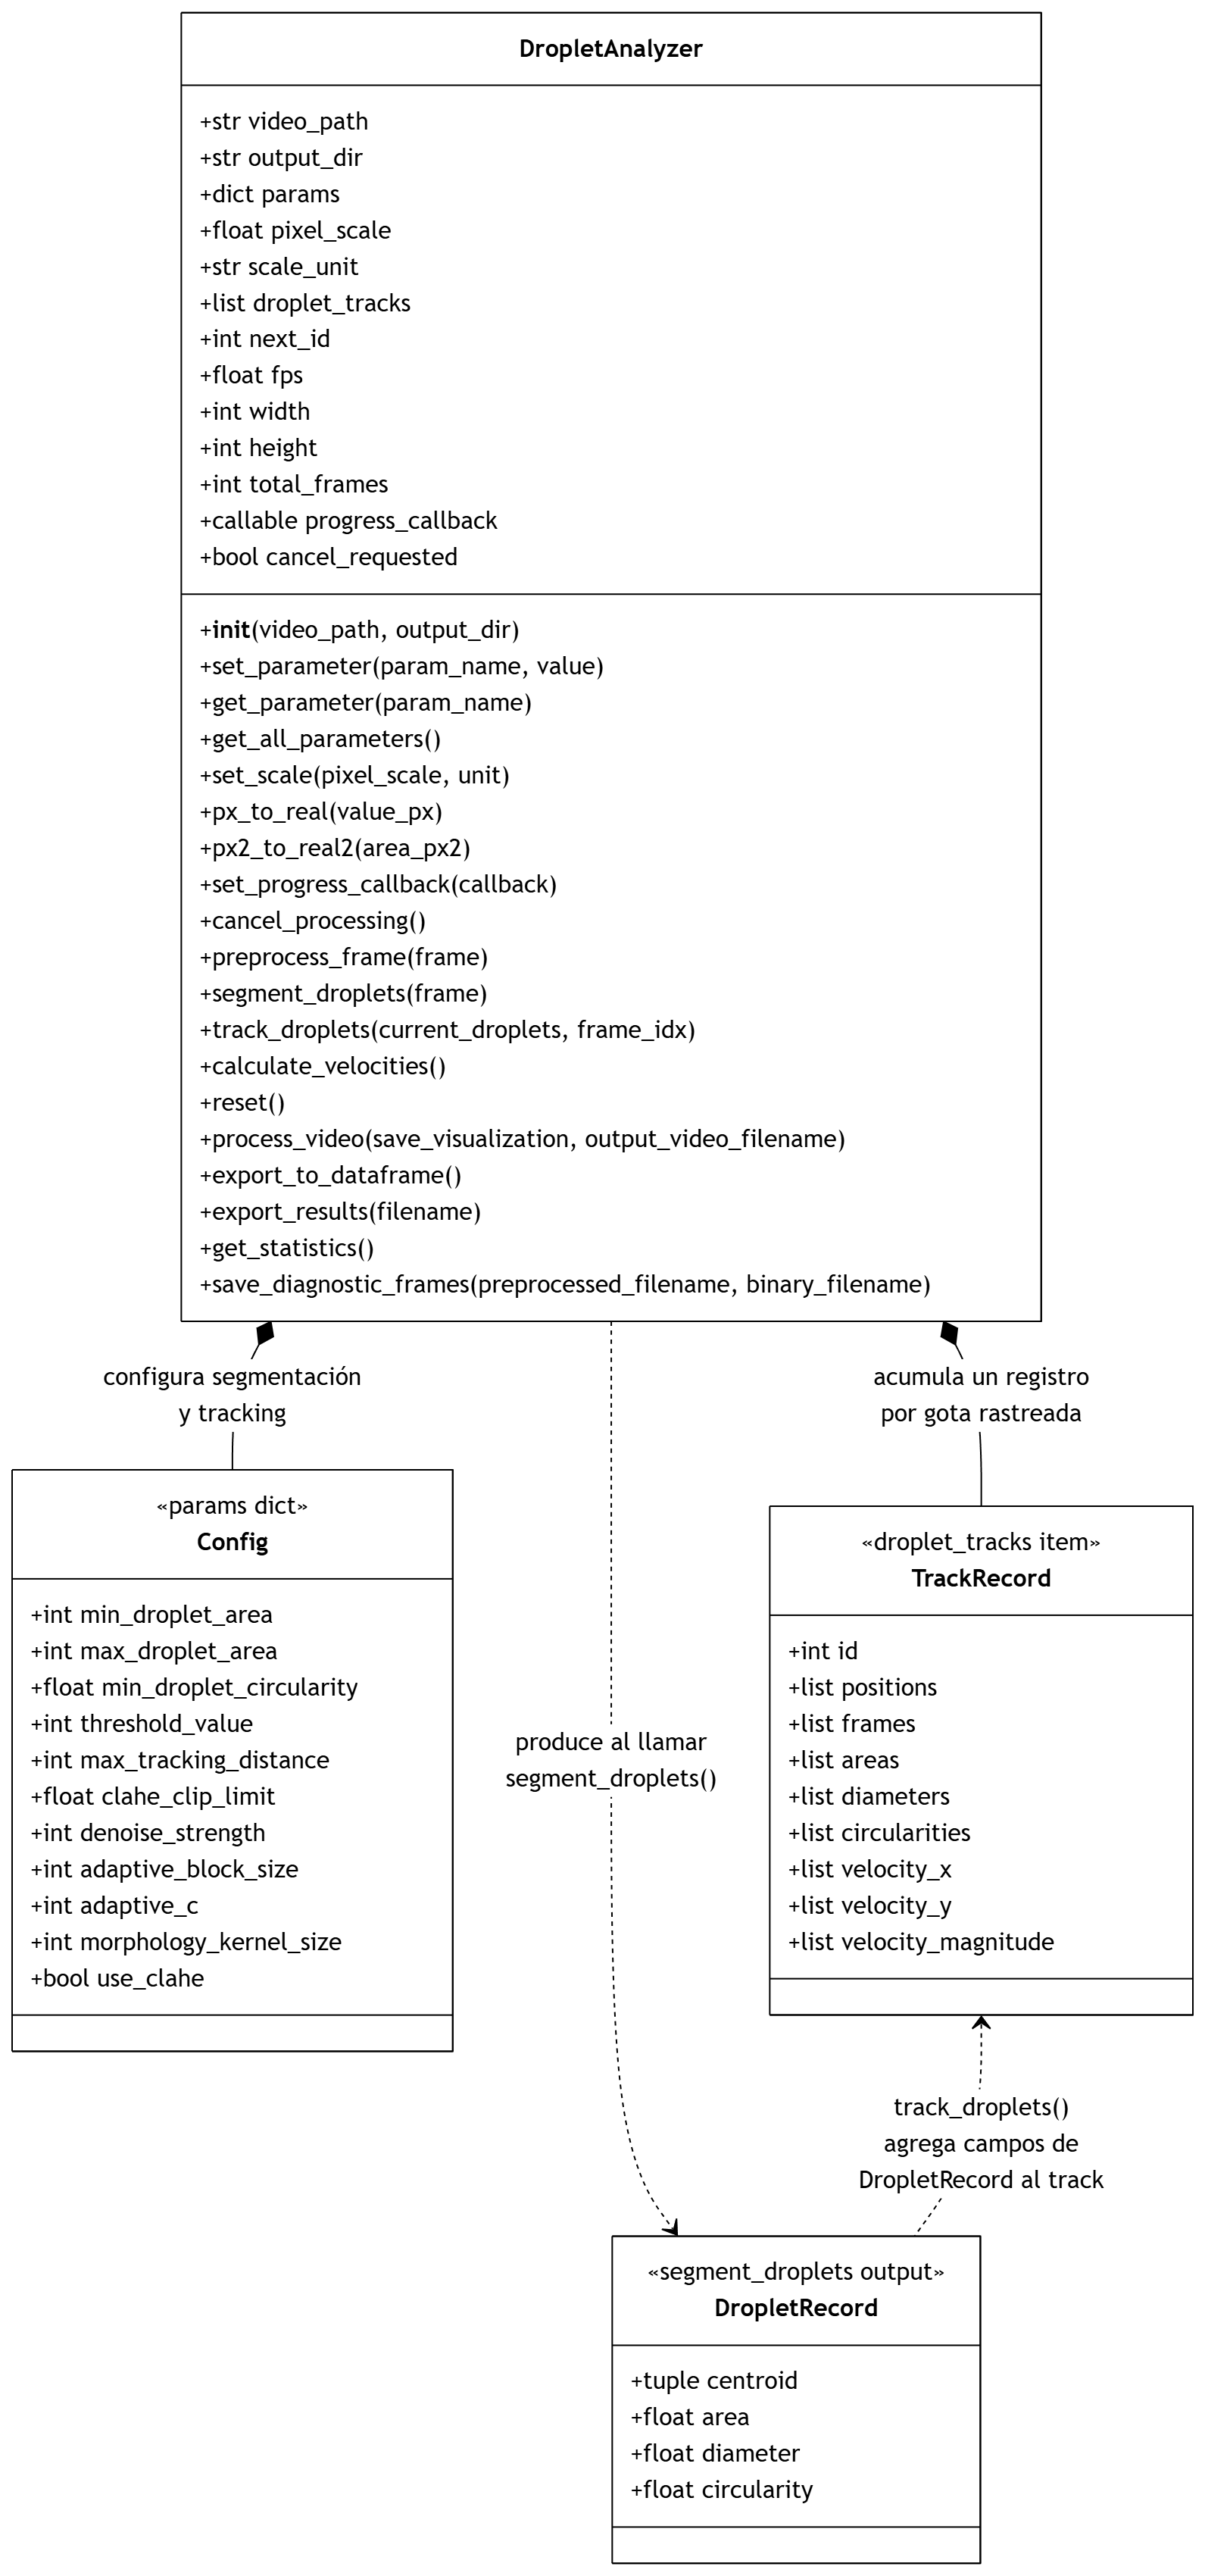
\includegraphics[width=0.7\textwidth]{figures/DiagramaClaseAn.png}
    \caption{Diagrama de la clase DropletAnalyzer.}
    \label{fig:diagramaClaseAn}
\end{figure}
\FloatBarrier

\subsubsection{Mejora del contraste}

Gran parte de los frames capturados durante los experimentos presentan un bajo contraste, como se puede apreciar en la figura \ref{subfig:original}. Para mejorar esto, se han implementado dos técnicas que trabajan sobre sus histogramas: La ecualización adaptativa del histograma (CLAHE) \cite{zuiderveld1994clahe} y el estiramiento del histograma. La teoría detrás de estas técnicas se explicó en la sección \ref{subsec:preproc}, por lo que aquí nos centraremos en su implementación y resultados.

Para la implementación de CLAHE se ha usado la función \texttt{cv2.createCLAHE} de OpenCV, que permite configurar el tamaño de los tiles y el límite de contraste. En el caso del estiramiento del histograma, se ha implementado una función personalizada que ignora el 0.4\% de los píxeles más oscuros y el 0.4\% de los píxeles más claros, estirando el rango de intensidad entre estos percentiles.

El usuario tiene la capacidad de seleccionar entre estas dos técnicas de mejora de contraste y modificar algunos de sus parámetros desde la interfaz gráfica.

La implementación es la siguiente:
\\
\begin{lstlisting}[language=Python, caption={Implementación de mejora de contraste mediante CLAHE y estiramiento por percentiles.}, label={lst:mejora-contraste}]
if self.params['use_clahe']:
    clh = cv2.createCLAHE(
        clipLimit=self.params['clahe_clip_limit'], 
        tileGridSize=(8, 8)
    )
    enhanced = clh.apply(gray)

else:
    flattened = gray.flatten()
    low_percentile = 0.4
    high_percentile = 100.0 - 0.4
    low_val, high_val = np.percentile(flattened, [low_percentile, high_percentile])
    dst = np.clip(gray, low_val, high_val)
    enhanced = ((dst - low_val) / (high_val - low_val) * 255).astype(np.uint8)
\end{lstlisting}

\begin{figure}[ht]
    \centering

    \begin{subfigure}[b]{0.45\textwidth}
        \centering
        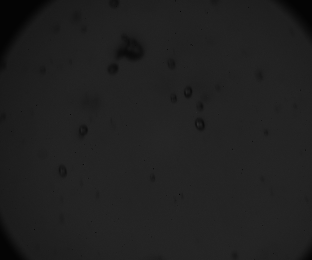
\includegraphics[width=\textwidth]{figures/frameoriginal.png}
        \caption{Original}
        \label{fig:original}
    \end{subfigure}
    \vspace{20pt} 
    \begin{subfigure}[b]{0.45\textwidth}
        \centering
        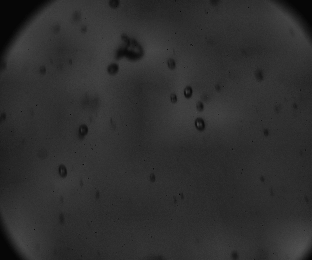
\includegraphics[width=\textwidth]{figures/CLAHE.png}
        \caption{CLAHE}
        \label{fig:CLAHE}
    \end{subfigure}
    \hfill 
    \begin{subfigure}[b]{0.45\textwidth}
        \centering
        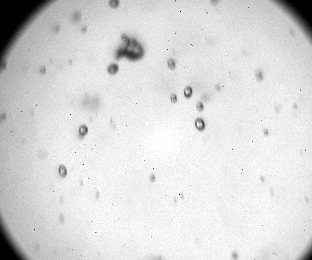
\includegraphics[width=\textwidth]{figures/contrasteporpercentil.png}
        \caption{Estiramiento del histograma}
        \label{fig:estiramiento}
    \end{subfigure}
    \caption{Comparación de técnicas de mejora de contraste.}
    \label{fig:mejora-contraste}
\end{figure}

En la figura \ref{fig:mejora-contraste} se puede apreciar la mejora del contraste obtenida con ambas técnicas. También se puede observar claramente que el estiramiento por percentiles es más agresivo, lo que puede ser beneficioso para algunos vídeos, pero también introduce más ruido, mientras que CLAHE es más suave y puede ser preferible para vídeos con menos problemas de contraste. Por otro lado, se puede apreciar que CLAHE se aplica de manera local, lo que genera esas pequeñas regiones más claras alrededor de las gotas, mientras que el estiramiento por percentiles se aplica de manera global, generando un fondo más uniforme.

\subsubsection{Reducción de ruido}

Tras aplicar las técnicas de mejora de contraste, se introduce algo de ruido de tipo sal y pimienta, como se puede apreciar en \ref{sub@fig:estiramiento}. Para reducir este ruido se ha optado por el uso del algoritmo Fast Non-Local Means Denoising \cite{ipol.2011.bcm_nlm}, implementado en OpenCV a través de la función \texttt{cv2.fastNlMeansDenoising}. Este algoritmo es una versión optimizada del algoritmo Non-Local Means, que reduce el ruido preservando los bordes y detalles de la imagen. El usuario puede configurar el parámetro de fuerza de reducción de ruido desde la interfaz gráfica, permitiendo ajustar el nivel de suavizado según las características específicas de cada vídeo. La teoría detrás de este algoritmo y de otras técnicas de reducción de ruido se explicaron en la sección \ref{subsec:preproc}.

Hay que remarcar que este paso es uno de los más complejos computacionalmente, pero dado que la solución no necesita ser en tiempo real, se ha optado por sacrificar algo de rendimiento a cambio de una mejor calidad en la segmentación de las gotas.

\begin{figure}[ht]
    \centering
    \begin{subfigure}[t]{0.45\textwidth}
        \centering
        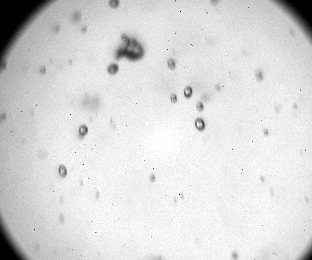
\includegraphics[width=\textwidth]{figures/contrasteporpercentil.png}
        \caption{Ruidosa tras estiramiento}  
        \label{subfig:originalDenoising}
    \end{subfigure}
    \hfill
    \begin{subfigure}[t]{0.45\textwidth}
        \centering
        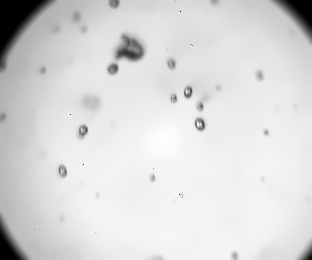
\includegraphics[width=\textwidth]{figures/denoisingNlMeans.png}
        \caption{Denoised}  
        \label{subfig:denoised}
    \end{subfigure}
    
    \caption{Reducción de ruido mediente FNL means Denoising ($h=10$).}
    \label{fig:denoising}
\end{figure}

Como se puede apreciar en la figura \ref{fig:denoising}, el algoritmo FNL means Denoising es capaz de reducir el ruido introducido por el estiramiento del histograma, preservando los bordes y detalles de las gotas. Sin embargo, también se puede observar que se pierde algo de detalle en las gotas más pequeñas, pero en general, las gotas enfocadas de mayor tamaño preservan su forma y bordes.

\subsection{Segmentación y filtrado}

Como se puede apreciar en el diagrama de la figura \ref{fig:diagramaPipeline}, esta etapa es la que conlleva un mayor número de pasos, y podríamos decir que es la etapa central del pipeline de procesamiento, ya que es la encargada de segmentar las gotas presentes en cada frame y extraer las características relevantes para el análisis posterior. En esta sección se describirán los algoritmos y técnicas seleccionados para cada uno de los bloques que componen esta etapa, así como los resultados obtenidos.

\subsubsection{Umbralización}

En este punto nos encontramos con una imagen preprocesada en escala de grises. Para conseguir segmentar las gotas necesitamos diferenciar los píxeles que pertenecen a las gotas de los que pertenecen al fondo. Para ello, se ha implementado una umbralización adaptativa gaussiana, que nos devuelve un frame binarizado, donde los píxeles blancos (255) corresponden a gotas y los píxeles negros (0) corresponden al fondo. 

De todas los algoritmos de umbralización explicados en \ref{subsec:segmentacion}, se ha escogido la umbralización por media local gaussiana, gracias a que al ser local, es mucho más robusta en imágenes que no poseen las mismas condiciones de iluminación en todas las regiones.

La implementación de este método se ha realizado utilizando el método \texttt{adaptiveThreshold} de la biblioteca OpenCV, tomando los parámetros de tamaño de bloque y C de la interfaz de usuario.
\\
\begin{lstlisting}[language=Python, caption=Implementación de Umbralización Adaptativa Gaussiana en OpenCV]
binary = cv2.adaptiveThreshold(
    denoised, 255,
    cv2.ADAPTIVE_THRESH_GAUSSIAN_C,
    cv2.THRESH_BINARY_INV,
    params['adaptive_block_size'],
    params['adaptive_c']
)
\end{lstlisting}

En la figura \ref{fig:thresholding} se puede apreciar el resultado de aplicar esta técnica, hay que destacar que, aún habiendo aplicado un proceso de denoising previo, se sigue observando algo de ruido de tipo sal y pimienta que se eliminará en los siguientes pasos. Quitando el ruido, se puede apreciar que las gotas enfocadas de mayor tamaño se segmentan correctamente, aunque las gotas más pequeñas y desenfocadas no se segmentan tan bien, lo que es un problema común en este tipo de vídeos. Sin embargo, el objetivo de esta etapa no es conseguir una segmentación perfecta, sino una segmentación lo suficientemente buena como para poder extraer características relevantes de las gotas y realizar un seguimiento posterior.

\begin{figure}[ht]
    \centering
    \begin{subfigure}[t]{0.45\textwidth}
        \centering
        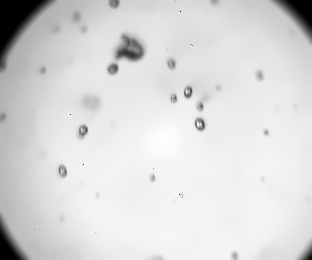
\includegraphics[width=\textwidth]{figures/denoisingNlMeans.png}
        \caption{Denoised}  
        \label{subfig:originalBinary}
    \end{subfigure}
    \hfill
    \begin{subfigure}[t]{0.45\textwidth}
        \centering
        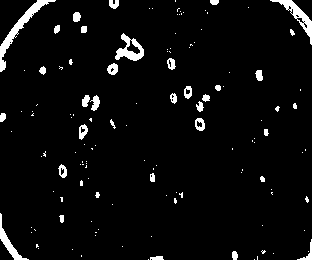
\includegraphics[width=\textwidth]{figures/bin.png}
        \caption{Binarizada}  
        \label{subfig:bin}
    \end{subfigure}
    
    \caption{Resultados de la umbralización adaptativa gaussiana.}
    \label{fig:thresholding}
\end{figure}

\subsubsection{Operaciones morfológicas}

Tras la umbralización, se han aplicado una serie de operaciones morfológicas para eliminar el ruido de tipo sal y pimienta presente en la imagen binarizada, así como para cerrar pequeños agujeros presentes en las gotas segmentadas. Para ello, se han implementado dos operaciones morfológicas: la apertura y el cierre, utilizando un kernel de forma elíptica de tamaño configurable desde la interfaz gráfica. La apertura se encarga de eliminar el ruido de tipo sal y pimienta, mientras que el cierre se encarga de cerrar pequeños agujeros presentes en las gotas segmentadas, mejorando así la calidad de la segmentación.
La implementación de estas operaciones se ha realizado utilizando la función \texttt{cv2.morphologyEx} de OpenCV, aplicando primero la apertura y luego el cierre.

El usuario puede configurar el tamaño del kernel utilizado en estas operaciones desde la interfaz gráfica, permitiendo ajustar el nivel de eliminación de ruido y cierre de agujeros según las características específicas de cada vídeo. Para ver la teoría detrás de estas operaciones morfológicas, se puede consultar \ref{subsec:segmentacion}.
\\
\begin{figure}[ht]
    \centering
    \begin{subfigure}[b]{0.45\textwidth}
        \centering
        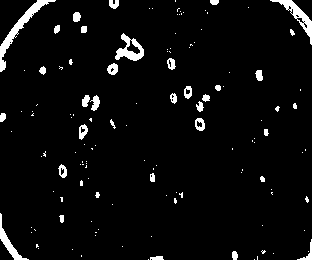
\includegraphics[width=\textwidth]{figures/bin.png}
        \caption{Binarizada}
        \label{fig:BinMorf}
    \end{subfigure}
    \hfill 
    \begin{subfigure}[b]{0.45\textwidth}
        \centering
        
\includegraphics[width=\textwidth]{figures/OPEN.png}
        \caption{Open}
        \label{fig:open}
    \end{subfigure}
    \vspace{20pt} 
    \begin{subfigure}[b]{0.45\textwidth}
        \centering
        
\includegraphics[width=\textwidth]{figures/CLOSE.png}
        \caption{Close}
        \label{fig:close}
    \end{subfigure}
    \caption{Resultados de las operaciones morfológicas.}
    \label{fig:morfologia}
\end{figure}

En la figura \ref{sub@fig:open} se aprecia que se ha limpiado gran parte del ruido tipo sal y pimienta, aunque también se abren pequeños huecos en la superficie de las gotas fruto de la erosión causada por la apertura. Dichos huecos se vuelven a cerrar tras aplicar la operación de cierre, como se aprecia en la figura \ref{sub@fig:close}.

\subsubsection{Extracción de contornos}

Una vez tenemos una imagen binarizada y lo más limpia posible, el siguiente paso es extraer los contornos de las gotas segmentadas. Para ello, se ha utilizado dos pasadas de la función \texttt{cv2.findContours} de OpenCV, que implementa el algoritmo de Suzuki \& Abe \cite{SUZUKI198532}, explicado en la sección \ref{subsec:segmentacion}.

En la primera pasada, se detectan los contornos de las gotas y se rellenan dichos contornos para obtener una máscara binaria rellena, que se utiliza para eliminar los huecos internos de las gotas segmentadas. En esta pasada se ha optado por usar el modo de recuperación de contornos \texttt{cv2.RETR\_EXTERNAL}, que solo recupera los contornos externos, ya que no nos interesa recuperar los contornos internos de las gotas, y el método de aproximación de contornos \texttt{cv2.CHAIN\_APPROX\_SIMPLE}, que comprime los contornos eliminando los puntos redundantes, ya que no necesitamos una representación exacta de los contornos en esta etapa, sino una representación aproximada que nos permita rellenar las gotas segmentadas.

En la segunda pasada, se vuelven a detectar los contornos sobre la máscara rellena, obteniendo así los contornos finales de las gotas segmentadas, que se utilizan para extraer las características relevantes de cada gota.
En esta pasada se ha optado por usar de nuevo el modo de recuperación de contornos \texttt{cv2.RETR\_EXTERNAL}, y el método de aproximación de contornos \texttt{cv2.CHAIN\_APPROX\_NONE}, que devuelve todos los puntos del contorno sin comprimir, ya que en esta etapa necesitamos una representación exacta de los contornos para poder extraer las características relevantes de cada gota.

\begin{figure}[ht]
    \centering
    \begin{subfigure}[b]{0.45\textwidth}
        \centering
        
\includegraphics[width=\textwidth]{figures/CLOSE.png}
        \caption{Close}
        \label{fig:closeCont}
    \end{subfigure}
    \hfill 
    \begin{subfigure}[b]{0.45\textwidth}
        \centering
        
\includegraphics[width=\textwidth]{figures/cont1.png}
        \caption{Pasada de rellenado}
        \label{fig:filling}
    \end{subfigure}
    \vspace{20pt} 
    \begin{subfigure}[b]{0.45\textwidth}
        \centering
        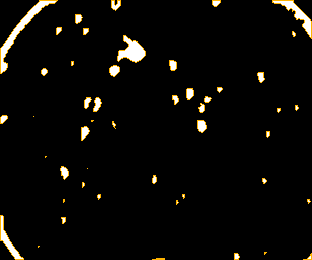
\includegraphics[width=\textwidth]{figures/cont2.png}
        \caption{Contornos finales}
        \label{fig:finalContours}
    \end{subfigure}
    \caption{Resultados de la extracción de contornos.}
    \label{fig:contornos}
\end{figure}

En la figura \ref{fig:contornos} se puede apreciar el resultado de la extracción de contornos. En la primera pasada, se detectan los contornos de las gotas segmentadas y se rellenan dichos contornos para obtener una máscara binaria rellena, que se muestra en la figura \ref{sub@fig:filling}. En la segunda pasada, se vuelven a detectar los contornos sobre la máscara rellena, obteniendo así los contornos finales de las gotas segmentadas, que se muestran en la figura de color naranja \ref{sub@fig:finalContours}.

\subsubsection{Filtro de área y circularidad}

En este paso se aplican dos filtros para eliminar los contornos que no corresponden a gotas, basándose en el área y la circularidad de los contornos detectados. 

\FloatBarrier
\section{Frontend}
